\section{Erläuterung des Fallbeispieles}
Ziel des Fallbeispieles ist es, ein Verfahren vom Entwurf bis zur Bereitstellung von containerisierten Microservices mit Kubernetes zu implementieren. Auf Basis dieses Verfahrens sollen Aussagen zur Umsetzung und dem Anwendungsgebiet getroffen werden können. Als Beispiel wird ein vereinfachtes \ac{CRM}-System verwendet. In diesem Kapitel werden die Vorgaben an das Fallbeispiel beschrieben.

\subsection{Anwendungseinsatz}
Ein \ac{CRM}-System ist eine Software für das Kundenbeziehungsmanagement. \ac{CRM}-Systeme sind komplexe betriebliche Anwendungssysteme. Durch ihre Größe und ihre vielen verwobenen Dienste gestaltet sich der Entwurf und die Weiterentwicklung häufig schwierig. \ac{CRM}-Systeme haben eine große fachliche Breite, was zu einem hohen Koordinationsaufwand bei der Entwicklung und der Bereitstellung führt \parencite[vgl.][S. 62]{trempArchitekturen2021}. Somit eignet sich ein \ac{CRM}-System als gutes Beispiel für die Umsetzung mit einer Microservice-Architektur, welche die Probleme weitgehend beheben soll. 

Das \ac{CRM}-System soll für das \ac{B2C} Umfeld entwickelt werden. Es soll bei der Verwaltung von Kontakten beziehungsweise Kunden helfen. Zu jedem Kontakt sollen Informationen und eine Historie mit allen Interaktionen abgespeichert werden. Darüber hinaus soll es auch möglich sein, Verkaufschancen zu verwalten und einem Kontakt zuzuordnen.

\subsection{Anwendungsfunktionen}
Die Kernfunktionalität des zu erstellenden \ac{CRM}-Systems ist das Anlegen, Anzeigen, Bearbeiten und Löschen von Kontakten, Interaktionen und Verkaufschancen. Konkret sollen die folgenden funktionalen Anforderungen von dem System erfüllt werden:
\begin{itemize}
\item Kontakte sollen mit Identifikationsnummer, Name, Geburtsdatum, Geschlecht, Telefonnummer, E-Mail-Adresse und Adresse angelegt, angezeigt, geändert und gelöscht werden können.
\item Interaktionen mit einem Kontakt sollen mit Identifikationsnummer, Art der Interaktion, Datum, Uhrzeit, Notizen und dem zugehörigen Kontakt angelegt, angezeigt, geändert und gelöscht werden können.
\item Mögliche Verkaufschancen sollen mit Identifikationsnummer, Status, voraussichtlichem Abschlussdatum, Verkaufswert, Rabatt, Budget des Kunden, Notizen und dem zugehörigen Kontakt angelegt, angezeigt, geändert und gelöscht werden können.
\end{itemize} 

Alle Funktionen sollen über eine einfache grafische Benutzeroberfläche mit dem Webbrowser bedienbar sein. Des Weiteren sollen alle Funktionen auch über \acp{API} angesteuert werden können, um die Integrierbarkeit mit anderen Systemen zu erleichtern. Durch die lose Kopplung einer Microservice-Architektur, soll eine flexible Skalierung und Erweiterbarkeit der Anwendung gewährleistet werden. Authentifizierung, Autorisierung und andere Sicherheitsfunktionen sollen nicht beachtet werden.

\clearpage
\section{Entwurf der Microservices}
In diesem Kapitel wird die Microservice-Architektur des \ac{CRM}-Systems entworfen. Dabei wird zuerst die Makro-Architektur des Gesamtsystems ausgearbeitet und anschließend die Mikro-Architektur der einzelnen Microservices festgelegt.

\subsection{Makro-Architektur}
Die Makro-Architektur muss besonders sorgfältig konzipiert werden, da Veränderungen auf dieser Ebene zu einem späteren Zeitpunkt sehr aufwendig werden können. Das Wichtigste ist eine gute fachliche Aufteilung der Microservices. Für die Aufteilung wird nach dem \ac{DDD} vorgegangen. Die Anwendung lässt sich in drei Bounded Contexts unterteilen: Kontaktverwaltung, Interaktionsverwaltung und Chancenverwaltung. Jeder dieser drei Bereiche besitzt ein eigenes Datenobjekt für einen Kontakt, eine Interaktion oder eine Chance. Eine Interaktion und eine Chance sollen einem Kontakt zuogeordnet werden können, deshalb benötigen diese Bounded Contexts einen Teil der Kontaktdaten. Die Identifikationsnummer eines Kontaktes reicht aus, um einer Interaktion oder Chance einen eindeutigen Kontakt zuzuordnen. Daraus ergibt sich die folgende Context Map, mit den drei Bounded Contexts und den Daten, an denen jeder Bounded Context interessiert ist. Anhand der identifizierten Kontextgrenzen wird die Anwendung in einen Kontakt-Microservice, einen Interaktions-Microservice und einen Chancen-Microservice aufgeteilt.

\begin{figure}[H] 
    \centering
    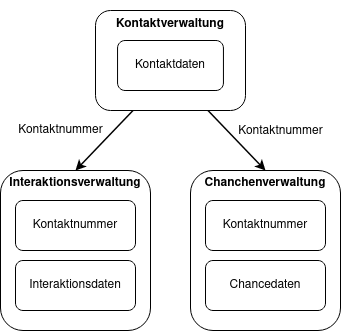
\includegraphics[width=0.60\textwidth]{figures/ContextMap.png}
    \caption{Context Map}
\end{figure}

Nachdem die fachliche Einteilung erledigt ist, kann jetzt die technischen Architektur festgelegt werden. Zur flexiblen Skalierbarkeit müssen die Microservices zustandslos sein. Alle persistenten Daten werden also in einer Datenbank abgelegt. Um eine möglichst große Unabhängigkeit zwischen den Microservices zu haben, wird jedem Microservice eine eigene Datenbank mit einem eigenen Datenbankschema zugeordnet. So können Datenstrukturen geändert werden, ohne unbeabsichtigte Auswirkungen auf andere Microservices zu haben. Der Interaktions-Microservice und der Chancen-Microservice benötigen für die Zuordnung zu einem Kontakt Informationen vom Kontakt-Microservice. Zwischen diesen Microservices ist somit eine Kommunikation nötig. Gibt es zu viele solcher Abhängigkeiten oder zyklische Aufrufe, sollte die Einteilung der Microservices überarbeitet werden. Das ist bei dieser Aufteilung jedoch nicht der Fall. Da alle Funktionalitäten auch über \acp{API} aufrufbar sein sollen, bietet es sich an, die Kommunikation zwischen den Microservices auch über diese \acp{API} abzuwickeln. Um die Microservices klein zuhalten, wird ein zentrales Frontend entwickelt werden, welches alle Funktionalitäten der Microservices bündelt. Um die Funktionalitäten zu integrieren, greift das Frontend auch auf die \acp{API} der Microservices zu. Somit ergibt sich der folgende Architekturentwurf aus drei verschiedenen Microservices mit drei zugehörigen Datenbanken und einem Frontend.

\begin{figure}[H] 
    \centering
    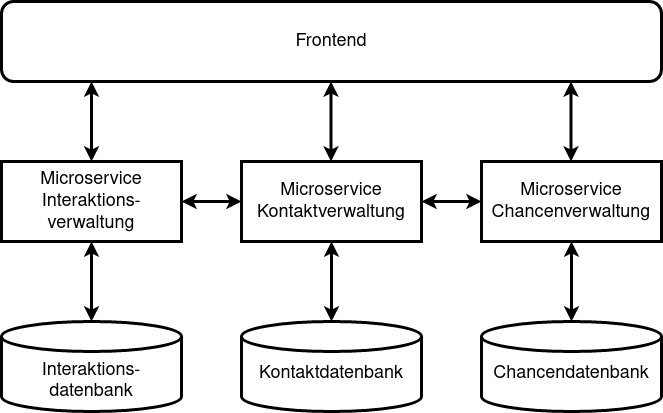
\includegraphics[width=0.8\textwidth]{figures/CRMEntwurf.png}
    \caption{Makro-Architektur des CRM-Systems}
\end{figure}

Als Nächstes müssen die \acp{API} der Microservices spezifiziert werden. Die \ac{API} wird nach dem \ac{REST}-Architekturstil entworfen. Die Kommunikation erfolgt dabei über \ac{HTTP}. Die \ac{REST}-Ressourcen sollen im \ac{JSON}-Format dargestellt werden. Für jeden Microservice werden die Endpunkte, unter der die \ac{API} aufrufbar ist und die HTTP-Anfragemethode bestimmt.

\begin{figure}[H] 
\centering
    \begin{tabularx}{\columnwidth}[H]{|p{45mm}|p{35mm}|X|}
    		\hline
        \rowcolor{lightgray!20}
        \textbf{Endpunkt} & \textbf{Methode} & \textbf{Beschreibung} \\
        \hline
        \hline
        \multicolumn{3}{|c|}{Kontakt-Microservice} \\
        \hline
        /contacts & GET & Gibt alle Kontakte zurück \\
        /contacts & POST & Fügt einen neuen Kontakt hinzu \\
        /contacts/\{ID\} & GET & Gibt einen Kontakt zurück \\
        /contacts/\{ID\} & PUT & Ändert einen Kontakt \\
        /contacts/\{ID\} & DELETE & Löscht einen Kontakt \\
        \hline
        \hline
        \multicolumn{3}{|c|}{Interaktions-Microservice} \\
        \hline
        /interactions & GET & Gibt alle Interaktionen zurück \\
        /interactions & POST & Fügt einen neue Interaktion hinzu \\
        /interactions/\{ID\} & GET & Gibt eine Interaktion zurück \\
        /interactions/\{ID\} & PUT & Ändert eine Interaktion \\
        /interactions/\{ID\} & DELETE & Löscht eine Interaktion \\
        \hline
        \hline
        \multicolumn{3}{|c|}{Chancen-Microservice} \\
        \hline
        /opportunity & GET & Gibt alle Chancen zurück \\
        /opportunity & POST & Fügt einen neue Chance hinzu \\
        /opportunity/\{ID\} & GET & Gibt eine Chance zurück \\
        /opportunity/\{ID\} & PUT & Ändert eine Chance \\
        /opportunity/\{ID\} & DELETE & Löscht eine Chance \\
        \hline
    \end{tabularx}
    \caption{Entwurf der REST-API}
\end{figure}

Service Discovery und Lastverteilung muss das System nicht selbst erledigen. Diese Funktionen werden von Kubernetes übernommen und erst bei der Bereitstellung konfiguriert.

\subsection{Mikro-Architektur}
Für das Gesamtsystem ist die Architektur eines einzelnen Microservice nicht von Bedeutung. Dadurch besitzt man bei der Gestaltung der Mikro-Architektur und vor allem bei der Auswahl des Technologie-Stacks viele Freiheiten. In diesem Fallbeispiel werden ausschließlich bewährte und beliebte Technologien eingesetzt. Die drei Microservices werden mit demselben Technologie-Stack und mit einer gleichartigen Architektur entworfen, um den Entwicklungsaufwand zu reduzieren. Es wäre aber auch möglich, alle Microservices mit verschiedenen Technologien zu implementieren, solange sie die gewünschten Schnittstellen anbieten können. Es wird Java in Verbindung mit dem Spring Boot Framework verwendet. Spring Boot bietet ein einsatzfertiges Baugerüst für Java-Anwendungen und eine einfache Auswahl von benötigten Abhängigkeiten, wie beispielsweise Datenbanktreibern. Auch \ac{REST}-\acp{API} werden von Spring Boot unterstützt. Spring Boot ist der De-Facto-Standard für Microservices in Java \parencite[vgl.][]{vmwareinc.Spring2022}. Für die Datenbanken wird MongoDB verwendet. MongoDB ist ein modernes dokumentorientiertes Datenbankmanagementsystem  \parencite[vgl.][]{mongodbinc.MongoDB2022}. Daten werden in Collections als Dokumente mit einem \ac{JSON}-ähnlichen Aufbau verwaltet. Die Datenstrukturen sind flexibel und können leichter umstrukturiert werden als bei klassischen Datenbanken. MongoDB wird auch als NoSQL-Datenbank bezeichnet.

Für alle drei Microservices werden Domänenmodelle erstellt. Die Domänenmodelle enthalten alle fachlichen Entitäten sowie deren Eigenschaften und Beziehungen. Für die Modellierung wird ein Klassendiagramm nach der \ac{UML} verwendet \parencite[vgl.][]{Unified2017}. \ac{UML} ist eine grafische Modellierungssprache, welche im Laufe der Arbeit noch häufiger eingesetzt wird. Die Domänenmodelle enhalten die gewünschten Eigenschaften aus den Anforderungen. Beim Kontakt-Microservice besteht das Datenmodell aus zwei Entitäten. Ein Kontakt besteht aus einer Adresse und mehreren anderen Eigenschaften, wie dem Namen, dem Geburtsdatum und einer Mail-Adresse. Da MongoDB eine NoSQL-Datenbank ist, besitzen die beiden Entitäten keine relationale Beziehung. Die Adresse wird verschachtelt im MongoDB-Dokument vom Kontakt abgespeichert werden. Des Weiteren enthält das Modell zwei Enumerationen für Auswahl des Geschlechts und der Nationalität.

\begin{figure}[H] 
    \centering
    \includegraphics[width=0.9\textwidth]{figures/DomänenmodellKontakt.png}
    \caption{Domänenmodell für den Kontakt-Microservice}
\end{figure} 

Das Datenmodell vom Interaktions-Microservice besteht lediglich aus einer einzelnen Entität und einer Enumeration für die Interaktionsart.

\begin{figure}[H] 
    \centering
    \includegraphics[width=0.9\textwidth]{figures/DomänenmodellInteraktion.png}
    \caption{Domänenmodell für den Interaktions-Microservice}
\end{figure}

Der Chancen-Microservice ist ähnlich aufgebaut und besitzt neben einer einzelnen Entität eine Enumeration für den Status einer Verkaufschance.

\begin{figure}[H] 
    \centering
    \includegraphics[width=0.9\textwidth]{figures/DomänenmodellChance.png}
    \caption{Domänenmodell für den Chancen-Microservice}
\end{figure}

Die einzelnen Microservices werden nach einer hexagonalen Architektur entworfen. Dabei handelt es sich um ein Architekturmuster bei der die Logik im Mittelpunkt steht. Sie hat verschiedene Schnittstellen (Ports), welche mit diversen Adaptern benutzt werden können. Das Architekturmuster wird deshalb auch als Ports and Adapters bezeichnet. Eine hexagonale Architektur ist eine Weiterentwicklung der klassischen Drei-Schichten-Architektur, bei der die Anwendung in eine Präsentationsschicht, eine Logikschicht und eine Datenhaltungsschicht aufgeteilt wird.

\begin{figure}[H] 
    \centering
    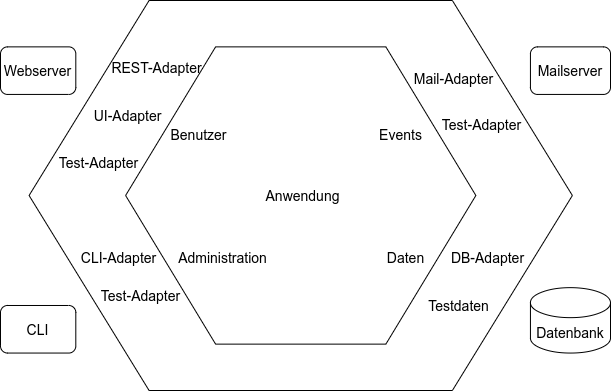
\includegraphics[width=0.9\textwidth]{figures/HexagonalDesignConcept.png}
    \caption{Überblick einer hexagonalen Architektur \parencite[vgl.][S. 204]{wolffMicroservices2018}}
\end{figure}

Jede Facette der Anwendung, wie Benutzer, Daten oder Admin ist ein Port, welcher von den Adaptern auf Technologien wie \ac{REST} umgesetzt wird \parencite[vgl.][S. 204]{wolffMicroservices2018}. Die Logik der Anwendung wird klar abgetrennt und nur die Adapter ermöglichen eine Kommunikation nach Außen. Dadurch bleibt der fachliche Code unabhängig vom technischen Code. Für das Fallbeispiel wird lediglich ein Port für die Daten und ein Port für die Benutzung benötigt. Zusätzlich wird ein Adapter für die \ac{REST}-\ac{API} und ein Adapter für MongoDB benötigt.

Als Frontend wird eine clientseitige Webanwendung eingesetzt. Diese wird mithilfe der JavaScript-Bibliothek React implementiert. React ist die beliebteste Bibliothek zum Erstellen von Web-\acp{UI} \parencite[vgl.][]{stackoverflowMost2021}. Anwendungen werden dabei aus wiederverwendbaren Komponenten zusammengesetzt werden, welche effizient gerendert und aktualisiert werden. Die Komponenten können sowohl aus JavaScript, \ac{HTML} und \ac{CSS} bestehen. 

\clearpage
\section{Implementierung}
In diesem Kapitel wird der erstellte Entwurf implementiert. Zuerst werden die Microservices angefertigt und anschließend das Frontend. Es sei auch erwähnt, dass der vollständige Quellcode unter dem folgenden GitHub Repository einsehbar ist: \href{https://github.com/SimonHirner/bachelor-thesis}{github.com/SimonHirner/bachelor-thesis}.

\subsection{Microservices}
Die Umsetzung aller drei Microservices ist sehr ähnlich, deshalb wird die Implementierung hauptsächlich am Beispiel des Kontakt-Microservices erläutert. Als Erstes wird das erstellte Domänenmodelle für den Kontakt-Microservice implementiert. Jede Entität wird mit seinen Eigenschaften wird in Java als eine Klasse mit Attributen dargestellt. Die Endpunkte der spezifizierten \ac{REST}-\ac{API} werden in der Klasse ContactController erstellt. Dieser fungiert als ein Adapter im Sinne der hexagonalen Architektur. Er benötigt einen Port, mit dem er auf Funktionen der Geschäftslogik zugreifen kann. Dafür wird das Interface ContactService erstellt. Dieses definiert die Funktionalitäten der Geschäftslogik, implementiert sie aber noch nicht. Erst in der Klasse ContactServiceImpl wird das Interface implementiert und die eigentliche Geschäftslogik niedergeschrieben. Dadurch ist die Logik vom Controller, der sich um die Anfragen auf die REST-Schnittstelle kümmert, unabhängig. Einen Adapter für die Anbindung an MongoDB bringt Spring bereits mit. Es muss lediglich noch das Interface ContactRepository erstellt werden, welches als Port den Adapter mit der Geschäftslogik verbindet. Die Klassen ContactController und ContactServiceImpl werden vollständig im \nameref{anhang} aufgelistet.

\begin{figure}[H] 
    \centering
    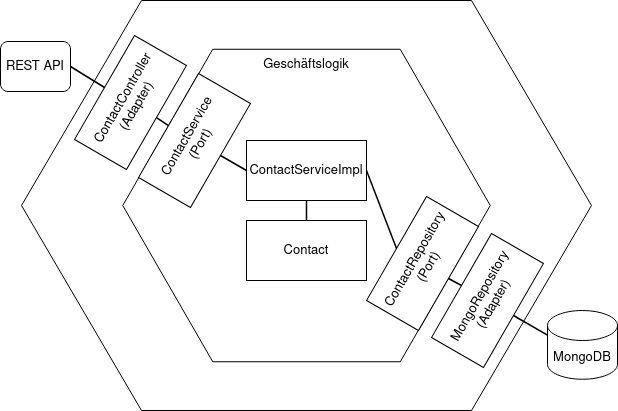
\includegraphics[width=0.9\textwidth]{figures/HexagonalDesign.png}
    \caption{Implementierung der hexagonalen Architektur beim Kontakt-Microservice}
\end{figure}

Den Mittelpunkt des Microservices bildet die Klasse ContactServiceImpl. Sie enthählt den Code, der die Geschäftslogik beschreibt. Die Klasse enthält verschiedene Methoden, um Kontakte zurückzugeben, zu löschen, zu speichern und zu ersetzen.

\begin{figure}[H] 
    \centering
    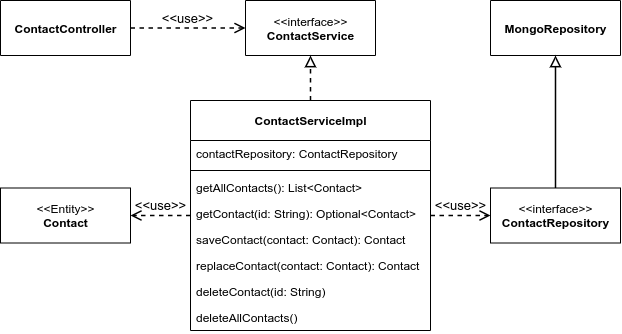
\includegraphics[width=0.9\textwidth]{figures/UMLKlassenDiagrammKontakt.png}
    \caption{Struktur vom Kontakt-Microservice}
\end{figure}

Der Interaktions-Microservice und der Chancen-Microservices unterscheiden sich bei der Geschäftslogik vom Kontakt-Microservice. Der Interaktions-Microservice muss beim Speichern einer Interaktion überprüfen, ob die Kontaktidentifikationsnummer der Interaktion gültig ist. Dafür ruft der Interaktions-Microservice den Kontakt-Microservice über seine \ac{REST}-\ac{API} auf und testet, ob zu der angegebenen Kontaktidentifikationsnummer ein Kontakt vorhanden ist. Das folgende \ac{UML}-Sequenzdiagramm zeigt den zeitlichen Verlauf der \ac{API}-Anfragen und die involvierten \ac{API}-Endpunkte. Da bei einer Chance auch eine Kontaktidentifikationsnummer angegeben werden kann, wird beim Chancen-Microservice dieselbe Logik implementiert.

\begin{figure}[H] 
    \centering
    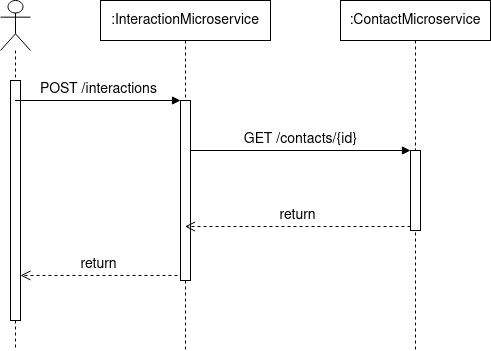
\includegraphics[width=0.75\textwidth]{figures/UMLSequenzdiagramm.png}
    \caption{Kommunikationsablauf zwischen Interaktions-Microservice und Kontakt-Microservice}
\end{figure}

Des Weiteren wird Swagger in die Microservices integriert. Bei Swagger handelt es sich ein Werkzeug zur sprachunabhängigen Spezifikation von \acp{API} \parencite[vgl.][]{smartbearsoftwareSwagger2022}. Swagger kann durch eine Abhängigkeit unkompliziert zu Spring Boot hinzu gefügt werden. Es erstellt automatisch eine Webseite mit einer Dokumentation der \ac{REST}-\ac{API}. 

\begin{figure}[H] 
    \centering
    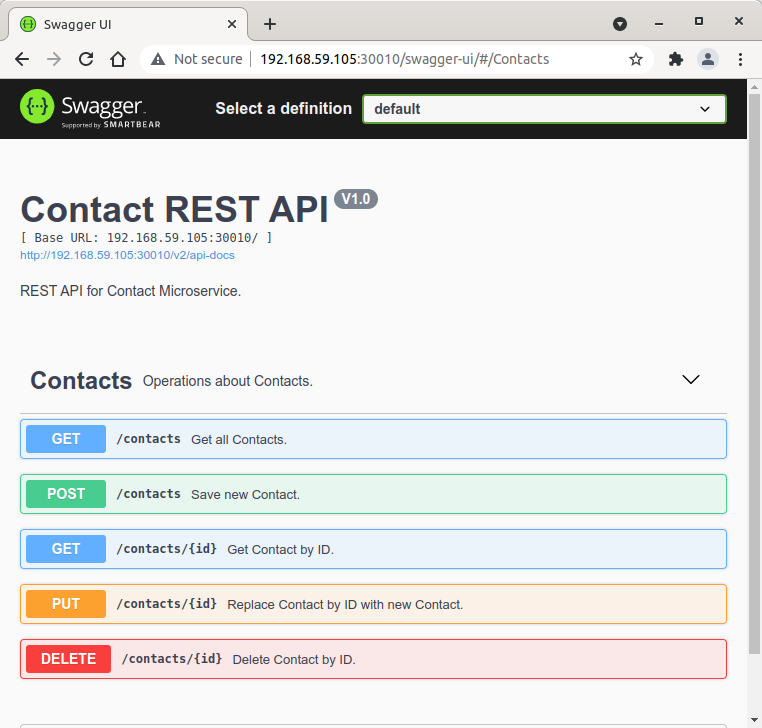
\includegraphics[width=0.9\textwidth]{figures/KontaktAPISwagger.png}
    \caption{Swagger Dokumentation der Kontakt-API}
\end{figure}

Alle drei Microservices benötigen die Adresse ihrer Datenbank, um mit ihr eine Verbindung aufzubauen. Der Interaktions-Microservice und der Verkaufschancen-Microservice brauchen darüber hinaus die Adresse des Kontakt-Microservices, um mit diesem zu kommunizieren. Diese Verbindungsinformationen werden den Anwendungen über Umgebungsvariablen übergeben. Später bei der Bereitstellung können so die Umgebungsvariablen der Container mit den richtigen Adressen besetzt werden.

\subsection{Frontend}

Das Frontend besteht aus insgesamt zehn verschiedenen Webseiten. Für jeden Kontakt, jede Interaktion und jede Verkaufschance gibt es jeweils eine Seite zum Einsehen aller Objekte, eine Seite zum Einsehen sowie Bearbeiten eines Objektes und eine Seite zum Anlegen eines neuen Objektes. Dazu hat das Frontend noch eine Startseite. Die Seiten setzen sich auch verschiedenen wiederverwendbaren Komponenten, wie beispielsweise der Navigationsleiste, Formularen und Tabellen zusammen. Die \ac{API}-Aufrufe werden über Funktionen in Service-Klassen implementiert, die von den Komponenten aufgerufen werden. Daraus ergibt sich der folgenden Aufbau für das Frontend.

\begin{figure}[H] 
    \centering
    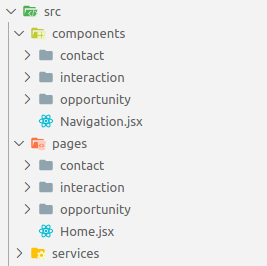
\includegraphics[width=0.5\textwidth]{figures/AufbauFrontend.png}
    \caption{Aufbau des Frontends}
\end{figure}

Zum Styling der Anwendung wird das CSS-Framework Bootstrap verwendet. Bei der Erstellung oder Bearbeitung einer Chance oder Interaktion kann über eine Dropdown-Liste ein zugehöriger Kontakte ausgewählt werden. Bei der Detailansicht eines Kontaktes wird neben den Attributen auch die zugehörigen Interaktionen und Verkaufschancen angezeigt. Im \nameref{anhang} finden sich Bildschirmfotos der beschriebenen Seiten. Auch ist dort eine der Service-Klassen zu finden, welche die Anfragen auf den Kontakt-Microservice regelt. Das Frontend benötigt die Adresse aller Services. Auch hier werden die Verbindungsinformationen über eine Umgebungsvariable übergeben. Bei React werden Umgebungsvariablen in die Datei .env.production geschrieben, da der Code des Frontends clientseitig ausgeführt wird.

\clearpage
\section{Bereitstellung mit Kubernetes}

Im letzten Teil des Fallbeispieles wird das fertige \ac{CRM}-System mit Kubernetes bereitgestellt. Dafür wird Docker, Minikube und Kubectl benötigt.

\subsection{Containerisierung}

Um die Microservices und das Frontend in Pods in einem Kubernetes Cluster laufen zu lassen, müssen sie erst mit Docker containerisiert werden. Dazu wird als Erstes ein Dockerfile für jeden Microservice erstellt. Anschließend kann aus dem Dockerfile ein Docker Image gebaut werden, mit dem dann ein entsprechender Container gestartet werden kann.

Dockerfiles besitzen eine eigene Syntax. Ein großgeschriebener Befehl wird gefolgt von einem oder mehreren Parametern. Es ähnelt einer Anleitung, welche Schritt für Schritt abgearbeitet wird. Die Dockerfiles der Microservices haben alle einen analogen Aufbau. Der erste Befehl in den Dockerfiles bestimmt, auf welchem Docker Image das neue Image basieren soll. Für die Microservices wird ein Image mit einer Java-Plattform verwendet, welches automatisch aus dem öffentlichen DockerHub heruntergeladen wird. Anschließend wird die \acs{JAR}-Datei der Anwendung in das Image kopiert. Als letzter Befehl wird festgelegt, dass die \acs{JAR}-Datei beim Start des Containers ausgeführt werden soll.

\begin{lstlisting}[language=dockerfile, caption=Dockerfile für den Kontakt-Microservice]
FROM openjdk:11-jdk-slim
ARG JAR_FILE=target/*.jar
COPY ${JAR_FILE} app.jar
EXPOSE 8080
ENTRYPOINT ["java","-jar","/app.jar"]
\end{lstlisting}

Das Frontend benötigt ein eigenes Dockerfile. Dieses hat einen mehrstufigen Aufbau. In der ersten Stufe, der Build-Stage, wird die React-Anwendung gebaut. Um die fertig gebaute Webanwendung an einen Browser auszuliefern wird ein Webserver benötigt. Die zweite Stufe des Dockerfiles basiert auf einem Image mit dem Webserver Nginx. Die React-Anwendung aus der Build-Stage wird nun in das finale Image kopiert.

\begin{lstlisting}[language=dockerfile, caption=Dockerfile für das Frontend]
FROM node:alpine as build
WORKDIR /app
COPY package*.json ./
RUN npm install --silent
COPY . .
RUN npm run build

FROM nginx:alpine
WORKDIR /usr/share/nginx/html
RUN rm -rf ./*
COPY --from=build /app/build .
ENTRYPOINT ["nginx", "-g", "daemon off;"]
\end{lstlisting}

Für die Datenbanken müssen keine eigenen Dockerfiles erstellt werden. Hier reichen unveränderte Images aus, welche vom DockerHub heruntergeladen werden können. Mit dem folgenden Befehl kann aus den erstellten Dockerfiles nun ein Docker Image gebaut werden.

\begin{lstlisting}[language=bash, caption=Docker-Befehl für das Bauen eines Images, captionpos=b]
docker build -t contact-microservice:latest .
\end{lstlisting}

\subsection{Bereitstellung}

Die fertigen Images können jetzt eingesetzt werden. Dazu wird zuerst das Kubernetes Cluster mit Minikube gestartet. Anschließend werden YAML-Dateien erstellt, in denen die gewünschten Kubernetes Objekte beschrieben werden. Für alle drei Microservices, alle drei Datenbanken und das Frontend muss jeweils ein Service und ein Deployment erstellt werden. In den Deployment-Objekten wird der Name der zuvor gebauten Images angegeben. Mit dem Attribut Replicas kann zudem die Anzahl der Pods, welche von einem Microservice gleichzeitig laufen sollen verändert werden. Bei den Microservices wird zudem die Adresse, unter der die Datenbank erreichbar ist, als Umgebungsvariable übergeben. Als Adresse wird der Name vom Service-Objekt der entsprechenden Datenbank verwendet werden.

\begin{lstlisting}[language=YAML, caption=Deployment-Objekt vom Kontakt-Microservice]
apiVersion: apps/v1
kind: Deployment
metadata:
  name: contact-service
spec:
  replicas: 1
  template:
    metadata:
      labels:
        app: contact-service
    spec:
      containers:
        - name: contact-service
          image: contact-microservice:latest
          imagePullPolicy: IfNotPresent
          ports:
          - containerPort: 8080
          env:
            - name: MONGODB_HOST
              value: contact-service
              valueFrom:
                configMapKeyRef:
                  name: contact-db-config  
                  key: host
\end{lstlisting}

Die Service-Objekte der Datenbanken sind vom Typ ClusterIP, da sie nur innerhalb des Clusters aufgerufen werden.
Die Service-Objekte der Microservices sind dagegen vom Typ NodePort. Somit kann ein fester Port angegeben werden, unter dem der Service auch von außerhalb des Clusters erreichbar ist. Anfragen auf einen Service werden automatisch von Kubernetes auf die Pods, welche dem Service zugeordnet sind, verteilt. 

\begin{lstlisting}[language=YAML, caption=Service-Objekt vom Kontakt-Microservice, captionpos=b]
kind: Service
apiVersion: v1
metadata:
  name: contact-service
spec:
  selector:
    app: contact-service
  ports:
  - protocol: TCP
    port: 8080
    nodePort: 30010
  type: NodePort
\end{lstlisting}

Sämtliche erstellte YAML-Dateien müssen über einen Kubectl-Befehl auf das Cluster angewendet werden. Kubernetes arbeitet dann automatisch die nötigen Schritte, um die beschriebenen Objekte zu erstellen.

\begin{lstlisting}[language=bash, caption=Kubectl-Befehl für das Anwenden einer YAML-Datei, captionpos=b]
kubectl apply -f contact-microservice.yaml
\end{lstlisting}

\subsection{Skalierung}
Um die Vorteile von der Microservices auszunutzen, soll die Anzahl der gleichzeitig laufenden Pods eines Microservices flexibel verwaltet werden. Abhängig von der Auslastung soll so eine horizontale Skalierung vorgenommen werden. Auch dafür wird eine YAML-Datei erstellt, in der ein \ac{HPA}-Objekt für jeden Microservice beschrieben wird. In der Datei wird angegeben, welches Deployment skaliert werden soll. Als Metrik für die Skalierung, wird die CPU-Auslastung des Pods verwendet. Darüber hinaus wird angegeben wie viele Pods vom entsprechenden Microservice minimal und maximal ausgeführt werden sollen.

\begin{lstlisting}[language=YAML, caption=HPA-Objekt vom Kontakt-Microservice, captionpos=b]
apiVersion: autoscaling/v1
kind: HorizontalPodAutoscaler
metadata:
    name: contact-service
spec:
    scaleTargetRef:
        apiVersion: apps/v1
        kind: Deployment
        name: contact-service
    minReplicas: 2
    maxReplicas: 4
    targetCPUUtilizationPercentage: 80
\end{lstlisting}

Nun ist die Bereitstellung abgeschlossen. Minikube bietet ein browserbasiertes Dashboard an, mit dem der Status des Clusters auch grafisch überprüft werden kann. Ein Bildschirmfoto des Dashboards kann im \nameref{anhang} gefunden werden. Das folgende Verteilungsdiagramm zeigt das Ergebnis der durchgeführten Bereitstellung.

\begin{figure}[H] 
    \centering
    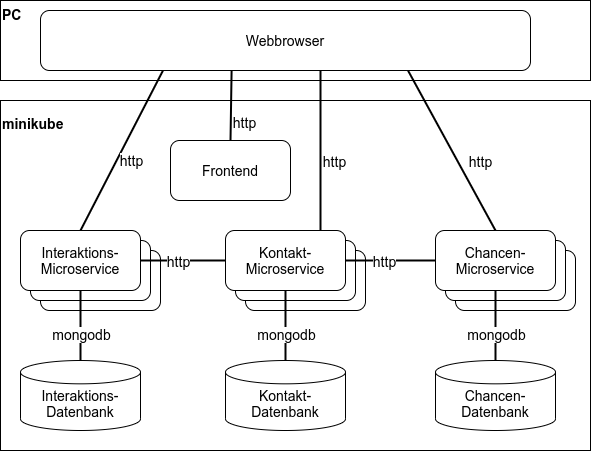
\includegraphics[width=0.82\textwidth]{figures/Verteilungsdiagramm.png}
    \caption{Verteilungsdiagramm}
\end{figure}
